%==============================================================
%  EE201 -- Circuit Theory I
%  Lecture 13 : Equivalent Resistances and Linearity -- slides
%  M. Mert Ankaralı, METU EEE
%
%  Compile:  ./build.sh      (or: pdflatex EE201_Lecture_13_slides.tex, twice)
%  Same colour code as the handout:
%      charge = purple, current = blue, voltage = orange, power = green
%==============================================================
\documentclass[11pt,aspectratio=169]{beamer}

\usepackage{appendixnumberbeamer}
\usepackage[T1]{fontenc}
\usepackage[utf8]{inputenc}
\usepackage[english]{babel}
\usepackage{lmodern}
\usepackage{amsmath,amssymb}
\usepackage{booktabs}
\usepackage{array}
\usepackage{colortbl}
\usepackage{tikz}
\usepackage[american,siunitx]{circuitikz}
\usetikzlibrary{matrix,arrows.meta,positioning,calc,decorations.pathreplacing,decorations.pathmorphing,decorations.markings}
\usetikzlibrary{overlay-beamer-styles}

%-------------------- plain METU-flavoured theme --------------
\usetheme{default}
\usecolortheme{default}
\useinnertheme{rectangles}
\setbeamertemplate{navigation symbols}{}
\setbeamertemplate{itemize items}[square]
\setbeamerfont{frametitle}{size=\large,series=\bfseries}
\setbeamerfont{title}{size=\LARGE,series=\bfseries}

\definecolor{metured}{RGB}{155,27,48}
\definecolor{metugray}{RGB}{88,89,91}
\definecolor{metulight}{RGB}{243,240,241}
\definecolor{ccur}{RGB}{0,102,170}
\definecolor{cvolt}{RGB}{214,120,0}
\definecolor{cpow}{RGB}{23,128,74}
\definecolor{ccharge}{RGB}{124,60,160}
\definecolor{cflux}{RGB}{0,138,138}
\definecolor{copper}{RGB}{184,98,30}

\setbeamercolor{structure}{fg=metured}
\setbeamercolor{frametitle}{fg=metured,bg=}
\setbeamercolor{title}{fg=metured}
\setbeamercolor{normal text}{fg=black!88}
\setbeamercolor{block title}{fg=white,bg=metured}
\setbeamercolor{block body}{bg=metulight}
\setbeamercolor{alerted text}{fg=metured}

\setbeamertemplate{frametitle}{%
  \vspace{0.55em}%
  \usebeamerfont{frametitle}\usebeamercolor[fg]{frametitle}\insertframetitle\par
  \vspace{-0.2em}{\color{metured}\rule{\textwidth}{1pt}}\par\vspace{-0.2em}}

\setbeamertemplate{footline}{%
  \hbox{\begin{beamercolorbox}[wd=\paperwidth,ht=2.4ex,dp=1.4ex,leftskip=1.2em,rightskip=1.2em]{}%
  \tiny\color{metugray}\coursecode\ \textbar\ Lecture 13: Equivalent Resistances and Linearity
  \hfill \insertframenumber/\inserttotalframenumber
  \end{beamercolorbox}}}

%-------------------- macros ----------------------------------
\newcommand{\coursecode}{EE201}
\newcommand{\term}{Fall 2026--2027}
\newcommand{\Icol}[1]{\textcolor{ccur}{#1}}
\newcommand{\Vcol}[1]{\textcolor{cvolt}{#1}}
\newcommand{\Pcol}[1]{\textcolor{cpow}{#1}}
\newcommand{\Qcol}[1]{\textcolor{ccharge}{#1}}
\newcommand{\Fcol}[1]{\textcolor{cflux}{#1}}
\newcommand{\uni}[1]{\,\mathrm{#1}}
\newcommand{\A}{\uni{A}} \newcommand{\V}{\uni{V}}
\newcommand{\W}{\uni{W}} \newcommand{\J}{\uni{J}}
\newcommand{\Cb}{\uni{C}} \newcommand{\s}{\uni{s}}
\newcommand{\Wb}{\uni{Wb}} \newcommand{\Hy}{\uni{H}}
\newcommand{\Sie}{\uni{S}}


%  voltage sources: smaller + and - inside the circle, further apart
\ctikzset{bipoles/vsourceam/inner plus={\tiny$+$},
          bipoles/vsourceam/inner minus={\tiny$\vphantom{+}-$},
          bipoles/vsourceam/margin=0.85,
          bipoles/cvsourceam/inner plus={\tiny$+$},
          bipoles/cvsourceam/inner minus={\tiny$\vphantom{+}-$},
          bipoles/cvsourceam/margin=0.85}
\ctikzset{bipoles/length=0.9cm, label/align=straight,
          bipoles/generic/height=0.28, bipoles/generic/width=0.62}
\tikzset{
  iar/.style={-{Stealth[length=2.2mm]}, ccur, thick},
  glab/.style={font=\footnotesize, text=metured},
  ttl/.style={font=\scriptsize\bfseries, text=metugray},
  capn/.style={font=\scriptsize, text=metugray, align=center},
  pol/.style={font=\small, text=cvolt},
  nlab/.style={circle, draw=metured, text=metured, font=\scriptsize, inner sep=0.7pt},
  blab/.style={font=\footnotesize, text=black!80},
  gbr/.style={black!75, thick, postaction={decorate, decoration={markings,
      mark=at position 0.56 with {\arrow{Stealth[length=2.5mm]}}}}},
  hal/.style={draw=cpow!60, line width=6pt, opacity=0.35, line cap=round, line join=round},
  halo/.style={circle, fill=metured!16, minimum size=0.95cm},
  elem/.style={draw=metugray, thick, fill=metulight},
  bigarr/.style={-{Stealth[length=3mm]}, very thick, metugray},
}

%-------------------- Lecture 13 circuit macros ---------------
\newcommand{\ohm}{\,\Omega}
\newcommand{\yes}{\textcolor{cpow}{\checkmark}}
\newcommand{\e}[1]{\textcolor{cvolt}{e_{#1}}}
\newcommand{\nd}[1]{\tikz[baseline=(c.base)]\node[nlab](c){#1};}
\newcommand{\nodev}[3]{\fill (#1) circle (1.7pt) node[#2, inner sep=2pt, font=\small, text=cvolt] {#3};}
\newcommand{\gnd}[2]{\draw (#1,#2) -- ++(0,-0.2) node[ground] {};}
\newcommand{\Rin}{R_{\mathrm{in}}}
%  Sum of the Delta resistors
\newcommand{\SD}{R_A + R_B + R_C}
\tikzset{tlab/.style={font=\small\bfseries, text=black!80},
         hterm/.style={circle, draw=metured, line width=1.6pt, minimum size=9pt, inner sep=0pt},
         sdel/.style={draw=metured, line width=5pt, opacity=0.25, line join=round, line cap=round},
         swye/.style={draw=ccur, line width=5pt, opacity=0.25, line join=round, line cap=round}}

%  A one-port N (box, text #1) with terminals a, b on the right; port current i into a, voltage v
\newcommand{\oneport}[2][1.9]{%
  \draw[elem] (0,0) rectangle (#1,2);
  \node[align=center, font=\small] at ({#1/2},1) {#2};
  \begin{scope}[shift={(#1-1.9,0)}]
  \draw (1.9,1.7) -- (3.0,1.7) node[ocirc] {} node[right, tlab] {a};
  \draw (1.9,0.3) -- (3.0,0.3) node[ocirc] {} node[right, tlab] {b};
  \draw[iar] (2.75,1.95) -- (2.2,1.95); \node[font=\small, text=ccur] at (2.48,2.2) {$i$};
  \node[pol] at (2.6,1.4) {$+$}; \node[pol] at (2.6,0.6) {$-$};
  \node[font=\small, text=cvolt] at (2.6,1.0) {$v$};
  \end{scope}}
%  A single resistor R_in between terminals a, b
\newcommand{\rinres}{%
  \draw (1.1,1.7) -- (0,1.7) to[R, l_=$\Rin$] (0,0.3) -- (1.1,0.3);
  \draw (1.1,1.7) node[ocirc] {} node[right, tlab] {a};
  \draw (1.1,0.3) node[ocirc] {} node[right, tlab] {b};}

%  Test source configurations.  #1 = 0: N with 1 A (I);  1: R_in with 1 A (II)
\newcommand{\testcfg}[1]{%
  \ifnum#1=0
    \draw[elem] (0,0) rectangle (1.5,2); \node at (0.75,1) {$N$};
    \draw (1.5,1.7) -- (2.9,1.7); \draw (1.5,0.3) -- (2.9,0.3);
    \draw (2.9,0.3) to[american current source, l_=$1\A$] (2.9,1.7);
    \node[pol] at (2.05,1.35) {$+$}; \node[pol] at (2.05,0.65) {$-$};
    \node[font=\small, text=cvolt] at (2.05,1.0) {$v_{\mathrm{I}}$};
    \fill (2.9,1.7) circle (1.6pt); \fill (2.9,0.3) circle (1.6pt);
  \else
    \draw (2.9,1.7) -- (0.5,1.7) to[R, l_=$\Rin$] (0.5,0.3) -- (2.9,0.3);
    \draw (2.9,0.3) to[american current source, l_=$1\A$] (2.9,1.7);
    \node[pol] at (1.75,1.35) {$+$}; \node[pol] at (1.75,0.65) {$-$};
    \node[font=\small, text=cvolt] at (1.75,1.0) {$v_{\mathrm{II}}$};
    \fill (2.9,1.7) circle (1.6pt); \fill (2.9,0.3) circle (1.6pt);
  \fi}

%  Example 13.1: a CCVS (3/2) i_x, 3 Ohm, 2 Ohm; port a-b on the right.
%  #1 = 0: bare, R_in = ?;  1: with the 1 A test source, the ground and e_1
\newcommand{\exR}[1]{%
  \draw (0,2) to[american controlled voltage source, l_=$\Vcol{\tfrac32\,i_x}$] (0,0);
  \draw (0,2) to[R, l=$3\ohm$] (2.4,2) to[R, l_=$2\ohm$] (2.4,0);
  \draw (2.4,2) -- (4.6,2); \draw (0,0) -- (4.6,0);
  \draw[iar] (4.3,0.28) -- (3.55,0.28); \node[font=\small, text=ccur] at (3.92,0.55) {$i_x$};
  \fill (2.4,2) circle (1.7pt); \fill (2.4,0) circle (1.7pt);
  \ifnum#1=0
    \draw (4.6,2) node[ocirc] {} node[above, tlab] {a};
    \draw (4.6,0) node[ocirc] {} node[below, tlab] {b};
    \draw[bigarr] (5.8,1) -- (4.9,1); \node[right] at (5.8,1) {$\Rin = \ ?$};
  \else
    \draw (4.6,0) to[american current source, l_=$1\A$] (4.6,2);
    \fill (4.6,2) circle (1.7pt); \fill (4.6,0) circle (1.7pt);
    \node[font=\small, text=cvolt, above] at (2.4,2.05) {$e_1$};
    \node[pol] at (3.75,1.65) {$+$}; \node[pol] at (3.75,0.95) {$-$};
    \node[font=\small, text=cvolt] at (3.75,1.3) {$v_{\mathrm{I}}$};
    \gnd{2.4}{0}
  \fi}

%  Three-terminal circuits.  Terminals A (0,0), B (3,0), C (1.5,2.5).
%  #1 = 0: no highlight;  1: A and B;  2: B and C;  3: C and A
\newcommand{\hlpair}[1]{%
  \ifcase#1\or
    \node[hterm] at (0,0) {}; \node[hterm] at (3,0) {};
  \or
    \node[hterm] at (3,0) {}; \node[hterm] at (1.5,2.5) {};
  \or
    \node[hterm] at (1.5,2.5) {}; \node[hterm] at (0,0) {};
  \fi}
%  Delta: R_C between A and B, R_A between B and C, R_B between C and A
\newcommand{\Dlt}[1]{%
  \draw (0,0) to[R] (3,0) to[R] (1.5,2.5) to[R] (0,0);
  \node[font=\small] at (1.5,-0.45) {$R_C$};
  \node[font=\small] at (2.85,1.6) {$R_A$};
  \node[font=\small] at (0.15,1.6) {$R_B$};
  \draw (0,0) node[ocirc] {} node[left=2pt, tlab] {A};
  \draw (3,0) node[ocirc] {} node[right=2pt, tlab] {B};
  \draw (1.5,2.5) node[ocirc] {} node[above=2pt, tlab] {C};
  \hlpair{#1}}
%  Y: R_1 at A, R_2 at B, R_3 at C, centre (1.5,0.95)
\newcommand{\Wye}[1]{%
  \draw (0,0) to[R] (1.5,0.95); \draw (3,0) to[R] (1.5,0.95);
  \draw (1.5,2.5) to[R] (1.5,0.95);
  \fill (1.5,0.95) circle (1.6pt);
  \node[font=\small] at (0.55,0.98) {$R_1$};
  \node[font=\small] at (2.45,0.98) {$R_2$};
  \node[font=\small] at (1.95,1.8) {$R_3$};
  \draw (0,0) node[ocirc] {} node[left=2pt, tlab] {A};
  \draw (3,0) node[ocirc] {} node[right=2pt, tlab] {B};
  \draw (1.5,2.5) node[ocirc] {} node[above=2pt, tlab] {C};
  \hlpair{#1}}
%  Equal resistors: #1 = 0: Delta with R, R, R;  1: Y with labels #2
\newcommand{\Dltq}{%
  \draw (0,0) to[R] (3,0) to[R] (1.5,2.5) to[R] (0,0);
  \node[font=\small] at (1.5,-0.45) {$R$};
  \node[font=\small] at (2.8,1.6) {$R$};
  \node[font=\small] at (0.2,1.6) {$R$};
  \foreach \p in {(0,0),(3,0),(1.5,2.5)} \draw \p node[ocirc] {};}
\newcommand{\Wyeq}[1]{%
  \draw (0,0) to[R] (1.5,0.95); \draw (3,0) to[R] (1.5,0.95);
  \draw (1.5,2.5) to[R] (1.5,0.95);
  \fill (1.5,0.95) circle (1.6pt);
  \node[font=\small] at (0.5,1.0) {$#1$};
  \node[font=\small] at (2.5,1.0) {$#1$};
  \node[font=\small] at (2.0,1.8) {$#1$};
  \foreach \p in {(0,0),(3,0),(1.5,2.5)} \draw \p node[ocirc] {};}

%  Example 13.2: a bridge between the terminals (top and bottom on the left).
%  #1 = 0: bare;  1: node names and the Delta A-B-C highlighted;  2: after Delta -> Y
\newcommand{\exBr}[1]{%
  \ifnum#1<2
    \draw (-1.3,4.0) -- (2,4.0) -- (2,3.4); \draw (-1.3,0) -- (2,0);
    \draw (-1.3,4.0) node[ocirc] {}; \draw (-1.3,0) node[ocirc] {};
    \draw (2,3.4) to[R] (0,1.7) to[R] (2,0);
    \draw (2,3.4) to[R] (4,1.7) to[R] (2,0);
    \draw (0,1.7) to[R] (4,1.7);
    \foreach \p in {(2,3.4),(0,1.7),(4,1.7),(2,0)} \fill \p circle (1.7pt);
    \node[font=\small] at (0.4,3.05) {$7\ohm$};
    \node[font=\small] at (3.6,3.05) {$20\ohm$};
    \node[font=\small] at (2,2.15) {$10\ohm$};
    \node[font=\small] at (0.4,0.3) {$50\ohm$};
    \node[font=\small] at (3.6,0.3) {$40\ohm$};
    \ifnum#1=1
      \draw[sdel] (0,1.7) -- (4,1.7) -- (2,0) -- cycle;
      \node[tlab, left] at (-0.1,1.7) {A}; \node[tlab, right] at (4.1,1.7) {B};
      \node[tlab, below right] at (2.05,-0.05) {C};
    \fi
  \else
    \draw (-1.3,4.0) -- (2,4.0) -- (2,3.4); \draw (-1.3,-0.6) -- (2,-0.6);
    \draw (-1.3,4.0) node[ocirc] {}; \draw (-1.3,-0.6) node[ocirc] {};
    \draw (2,3.4) to[R] (0,2.0) to[R] (2,0.9);
    \draw (2,3.4) to[R] (4,2.0) to[R] (2,0.9);
    \draw (2,0.9) to[R] (2,-0.6);
    \draw[swye] (0,2.0) -- (2,0.9) -- (4,2.0); \draw[swye] (2,0.9) -- (2,-0.6);
    \foreach \p in {(2,3.4),(0,2.0),(4,2.0),(2,0.9),(2,-0.6)} \fill \p circle (1.7pt);
    \node[font=\small] at (0.45,3.15) {$7\ohm$};
    \node[font=\small] at (3.6,3.15) {$20\ohm$};
    \node[font=\small, text=ccur] at (0.65,0.9) {$5\ohm$};
    \node[font=\small, text=ccur] at (3.35,0.9) {$4\ohm$};
    \node[font=\small, text=ccur] at (2.7,0.15) {$20\ohm$};
    \node[tlab, left] at (-0.1,2.0) {A}; \node[tlab, right] at (4.1,2.0) {B};
    \node[tlab, below right] at (2.05,-0.65) {C};
  \fi}

%  Example 13.3: v_s, R_1 (current i), R_2, i_s
\newcommand{\exL}{%
  \draw (0,2) to[american voltage source, l_=$\Vcol{v_s}$] (0,0);
  \draw (0,2) to[R, l=$R_1$] (3,2) to[R, l_=$R_2$] (3,0);
  \draw (3,2) -- (5.2,2); \draw (0,0) -- (5.2,0);
  \draw (5.2,0) to[american current source, l_=$\Icol{i_s}$] (5.2,2);
  \fill (3,2) circle (1.7pt); \fill (3,0) circle (1.7pt);
  \draw[iar] (1.1,1.55) -- (1.9,1.55); \node[font=\small, text=ccur] at (1.5,1.25) {$i$};}

%  Example 13.4: 20 V, 15 Ohm (i_x), 4 A, 10 Ohm (i), CCVS 5 i_x (+ at the bottom).
%  #1 = 0: all sources;  1: current source killed (open), i_1;  2: voltage source killed (short), i_2
\newcommand{\exS}[1]{%
  \ifnum#1=2
    \draw (0,2.2) -- (0,0);
    \node[font=\small, text=metured, rotate=90] at (-0.3,1.1) {short};
  \else
    \draw (0,2.2) to[american voltage source, l_=$\Vcol{20\V}$] (0,0);
  \fi
  \draw (0,2.2) to[R, l=$15\ohm$] (3.4,2.2) to[R, l=$10\ohm$] (6.8,2.2);
  \ifnum#1=1
    \draw (3.4,2.2) -- (3.4,1.75); \draw (3.4,0) -- (3.4,0.45);
    \draw (3.4,1.75) node[ocirc] {}; \draw (3.4,0.45) node[ocirc] {};
    \node[font=\small, text=metured] at (2.85,1.1) {open};
  \else
    \draw (3.4,0) to[american current source, l=$\Icol{4\A}$] (3.4,2.2);
  \fi
  \draw (6.8,0) to[american controlled voltage source, l_=$\Vcol{5\,i_x}$] (6.8,2.2);
  \draw (0,0) -- (6.8,0);
  \fill (3.4,2.2) circle (1.7pt); \fill (3.4,0) circle (1.7pt);
  \draw[iar] (0.6,1.8) -- (1.4,1.8); \node[font=\small, text=ccur] at (1.0,1.48) {$i_x$};
  \draw[iar] (4.6,1.8) -- (5.4,1.8);
  \node[font=\small, text=ccur] at (5.0,1.48) {\ifcase#1 $i$\or $i_1$\or $i_2$\fi};}

%  Example 13.5: v_s, R_1, CCVS r i_x (+ at the top), R_2 (voltage v), R_3 (current i_x), i_s
\newcommand{\exT}{%
  \draw (0,2) to[american voltage source, l_=$\Vcol{v_s}$] (0,0);
  \draw (0,2) to[R, l=$R_1$] (2.2,2) to[R, l=$R_2$] (4.8,2);
  \draw (2.2,2) to[american controlled voltage source, l_=$\Vcol{r\,i_x}$] (2.2,0);
  \draw (4.8,2) to[R, l_=$R_3$] (4.8,0);
  \draw (4.8,2) -- (6.6,2); \draw (0,0) -- (6.6,0);
  \draw (6.6,0) to[american current source, l_=$\Icol{i_s}$] (6.6,2);
  \foreach \p in {(2.2,2),(4.8,2),(2.2,0),(4.8,0)} \fill \p circle (1.7pt);
  \node[pol] at (2.85,1.62) {$+$}; \node[pol] at (4.15,1.62) {$-$};
  \node[font=\small, text=cvolt] at (3.5,1.62) {$v$};
  \draw[iar] (5.25,1.4) -- (5.25,0.7); \node[font=\small, text=ccur, anchor=west] at (5.3,1.05) {$i_x$};}

%  Linearity: block diagram
\newcommand{\blockdiag}{%
  \draw[elem] (0,0) rectangle (2.8,1.2);
  \node[align=center, font=\small] at (1.4,0.6) {LTI resistive\\circuit};
  \draw[-{Stealth[length=2.5mm]}, thick] (-1.5,0.6) -- (0,0.6) node[midway, above] {$\mathbf{u}$};
  \draw[-{Stealth[length=2.5mm]}, thick] (2.8,0.6) -- (4.3,0.6) node[midway, above] {$y$};
  \node[capn] at (-0.75,0.25) {input}; \node[capn] at (3.55,0.25) {output};}
\title{Lecture 13: Equivalent Resistances and Linearity}
\subtitle{EE201 -- Circuit Theory I}
\author{M. Mert Ankaralı}
\institute{\small Department of Electrical and Electronics Engineering\\
           Middle East Technical University}
\date{}

%  Roadmap icons, one per station (1-4)
\newcommand{\rmicon}[1]{%
  \ifcase#1\or
    \draw (0.9,0.6) -- (0,0.6) to[R] (0,-0.6) -- (0.9,-0.6);
    \draw (0.9,0.6) node[ocirc] {}; \draw (0.9,-0.6) node[ocirc] {};
    \node[font=\LARGE] at (-0.95,0) {$\Rin$};
  \or
    \draw (-1.1,-0.7) to[R] (1.1,-0.7) to[R] (0,1.0) to[R] (-1.1,-0.7);
  \or
    \draw[thick] (-0.8,-0.5) rectangle (0.8,0.5);
    \draw[-{Stealth[length=3mm]}, very thick] (-1.9,0) -- (-0.8,0);
    \draw[-{Stealth[length=3mm]}, very thick] (0.8,0) -- (1.9,0);
    \node[font=\LARGE] at (-1.4,0.45) {$\mathbf{u}$}; \node[font=\LARGE] at (1.4,0.45) {$y$};
  \or
    \draw (-2.0,-0.6) to[american voltage source] (-2.0,0.6) -- (-0.6,0.6) to[R] (-0.6,-0.6) -- (-2.0,-0.6);
    \node[font=\LARGE] at (0,0) {$+$};
    \draw (0.6,-0.6) to[american current source] (0.6,0.6) -- (2.0,0.6) to[R] (2.0,-0.6) -- (0.6,-0.6);
  \fi}
%  Stops 1-7: station of stop k = \rmst{k}
\newcommand{\rmst}[1]{\ifcase#1\or1\or2\or2\or2\or3\or4\or4\fi}
%  #1 station, #2 x, #3 title, #4 icon number
\newcommand{\rmstation}[4]{%
  \ifnum#1<\rmS\relax
    \node[circle, fill=cpow, text=white, inner sep=0pt, minimum size=5.4mm, font=\scriptsize\bfseries] at (#2,0) {\checkmark};
    \node[text=black!40, font=\bfseries] at (#2,0.62) {#3};
  \else\ifnum#1=\rmS\relax
    \node[circle, fill=metured, text=white, inner sep=0pt, minimum size=6.2mm, font=\small\bfseries] at (#2,0) {#1};
    \node[text=metured, font=\bfseries] at (#2,0.62) {#3};
  \else
    \node[circle, draw=metugray, fill=white, text=metugray, inner sep=0pt, minimum size=5.4mm, font=\scriptsize\bfseries] at (#2,0) {#1};
    \node[font=\bfseries] at (#2,0.62) {#3};
  \fi\fi
  \begin{scope}[shift={(#2,1.5)}, scale=0.42, transform shape]
    \ifnum#1>\rmS\relax\begin{scope}[opacity=0.5]\rmicon{#4}\end{scope}\else\rmicon{#4}\fi
  \end{scope}}
%  #1 first stop, #2 last stop covered by this item, #3 x, #4 y, #5 text
\newcommand{\rmsub}[5]{%
  \ifnum#2<\rmcur\relax
    \node[text width=3.05cm, align=center, font=\small, text=black!40] at (#3,#4) {#5\ \textcolor{cpow}{\checkmark}};
  \else\ifnum#1>\rmcur\relax
    \node[text width=3.05cm, align=center, font=\small] at (#3,#4) {#5};
  \else
    \node[text width=3.05cm, align=center, font=\small\bfseries, text=metured,
          draw=metured, rounded corners=2pt, inner sep=2pt] at (#3,#4) {#5};
  \fi\fi}
\newcommand{\roadmapframe}[1]{%
  \begin{frame}{Roadmap}
    \def\rmcur{#1}\edef\rmS{\rmst{#1}}%
    \vfill
    \centering
    \begin{tikzpicture}
      \draw[metugray!45, line width=3pt, -{Stealth[length=2.6mm, width=3.2mm]}] (0,0) -- (13.3,0);
      \rmstation{1}{1.75}{Input resistance}{1}
      \rmstation{2}{5.0}{$\boldsymbol{\Delta}$ and Y}{2}
      \rmstation{3}{8.45}{Linearity}{3}
      \rmstation{4}{11.65}{Superposition}{4}
      \rmsub{1}{1}{1.75}{-0.8}{a test source}
      \rmsub{1}{1}{1.75}{-1.55}{with a dependent source}
      \rmsub{2}{3}{5.0}{-0.8}{$\Delta$ to Y}
      \rmsub{2}{3}{5.0}{-1.45}{Y to $\Delta$}
      \rmsub{4}{4}{5.0}{-2.1}{a bridge}
      \rmsub{5}{5}{8.45}{-0.8}{$y = \mathbf{k}\,\mathbf{u}$}
      \rmsub{5}{5}{8.45}{-1.45}{the implication}
      \rmsub{6}{6}{11.65}{-0.8}{one source at a time}
      \rmsub{7}{7}{11.65}{-1.55}{three experiments}
    \end{tikzpicture}
    \vfill
    \mbox{}
    \vfill
  \end{frame}}
\begin{document}

%--------------------------------------------------------------
\begin{frame}[plain]
  \titlepage
  \vspace{-1.2em}
  \begin{center}\scriptsize\color{metugray}
    \Icol{$\blacksquare$}~current \quad \Vcol{$\blacksquare$}~voltage, node voltage $e$ \quad
    \textcolor{metured}{$\blacksquare$}~$\Delta$ \quad \Icol{$\blacksquare$}~Y
  \end{center}
\end{frame}

%--------------------------------------------------------------
\begin{frame}{Review: equivalent one-ports}
  \begin{columns}[c,onlytextwidth]
    \begin{column}{0.5\textwidth}
      \centering
      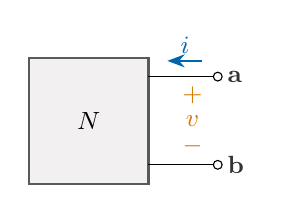
\begin{tikzpicture}[scale=0.8]
        \oneport{$N$}
      \end{tikzpicture}
    \end{column}
    \begin{column}{0.48\textwidth}
      \begin{itemize}\itemsep6pt
        \item One-port: a port $\Icol{i}$, $\Vcol{v}$
        \item<2-> Equivalent: the same $\Icol{i}$--$\Vcol{v}$ characteristic
        \item<3-> Series, parallel
        \item<3-> Source transformation
      \end{itemize}
    \end{column}
  \end{columns}
  \vfill
  \onslide<4->{%
  \begin{center}
    Node and mesh analysis: the \alert{original} circuit\\[4pt]
    Equivalents: a \alert{simpler} circuit
  \end{center}}
  \vfill
\end{frame}

%--------------------------------------------------------------
\begin{frame}{Motivation}
  \begin{columns}[t,onlytextwidth]
    \begin{column}{0.48\textwidth}
      \begin{block}{Dependent sources}
        \centering
        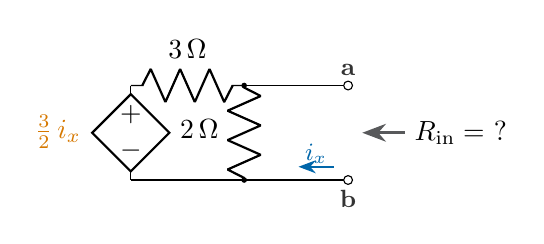
\begin{tikzpicture}[scale=0.6]
          \exR{0}
        \end{tikzpicture}\\[4pt]
        \raggedright
        Series, parallel: not enough
      \end{block}
    \end{column}
    \begin{column}{0.48\textwidth}
      \onslide<2->{%
      \begin{block}{A bridge}
        \centering
        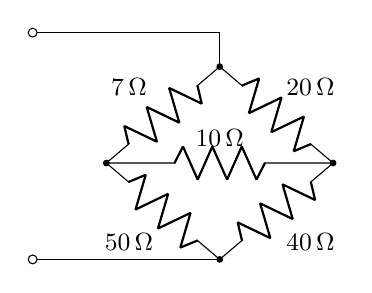
\begin{tikzpicture}[scale=0.72]
          \exBr{0}
        \end{tikzpicture}\\[4pt]
        \raggedright
        No series, no parallel
      \end{block}}
    \end{column}
  \end{columns}
  \vfill
  \onslide<3->{%
  \begin{center}
    One equivalent resistor in both? \ \onslide<4->{\alert{Yes}}
  \end{center}}
  \vfill
\end{frame}

%==============================================================
\roadmapframe{1}

%--------------------------------------------------------------
\begin{frame}{One-ports without independent sources}
  \vfill
  \begin{center}
    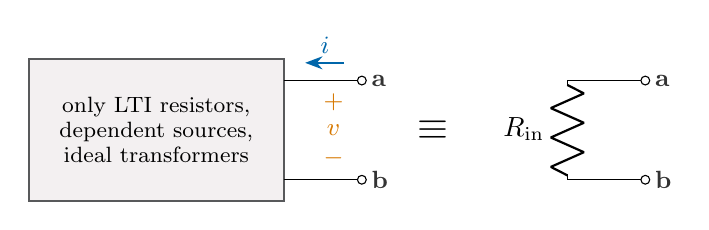
\begin{tikzpicture}[scale=0.9]
      \oneport[3.6]{\footnotesize only LTI resistors,\\[-2pt] \footnotesize dependent sources,\\[-2pt] \footnotesize ideal transformers}
      \node[font=\Large] at (5.7,1) {$\equiv$};
      \begin{scope}[shift={(7.6,0)}]
        \rinres
      \end{scope}
    \end{tikzpicture}
  \end{center}
  \vfill
  \begin{itemize}\itemsep8pt
    \item<2-> Controls of the dependent sources: \alert{inside} the one-port
    \item<3-> $\Vcol{v} = \Rin\,\Icol{i}$: \ $\Rin$ is the \alert{input resistance}
  \end{itemize}
  \vfill
\end{frame}

%--------------------------------------------------------------
\begin{frame}{Example 13.1: an input resistance}
  \vfill
  \begin{center}
    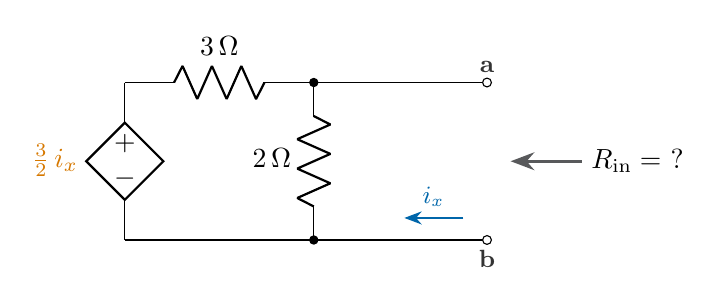
\begin{tikzpicture}[scale=1.0]
      \exR{0}
    \end{tikzpicture}
  \end{center}
  \vfill
\end{frame}

%--------------------------------------------------------------
\begin{frame}{The idea: a test source}
  \vfill
  \begin{columns}[c,onlytextwidth]
    \begin{column}{0.48\textwidth}
      \centering
      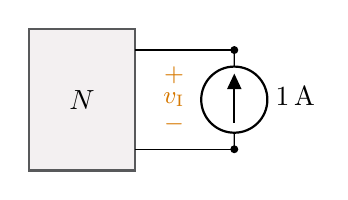
\begin{tikzpicture}[scale=0.9]
        \testcfg{0}
      \end{tikzpicture}\\[4pt]
      (I)
    \end{column}
    \begin{column}{0.48\textwidth}
      \centering
      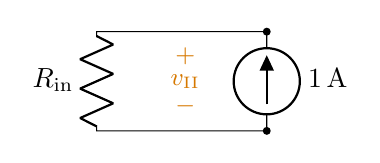
\begin{tikzpicture}[scale=0.9]
        \testcfg{1}
      \end{tikzpicture}\\[4pt]
      (II)
    \end{column}
  \end{columns}
  \vfill
  \onslide<2->{\begin{center}$N \equiv \Rin$ \ $\Rightarrow$ \ $\Vcol{v_{\mathrm{I}}} = \Vcol{v_{\mathrm{II}}} = \Rin \cdot 1\A$\end{center}}
  \vfill
  \onslide<3->{%
  \begin{center}
    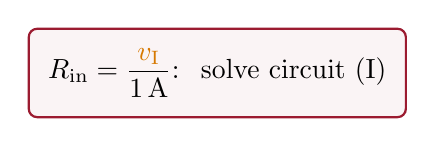
\begin{tikzpicture}
      \node[draw=metured, thick, fill=metured!5, rounded corners=3pt, inner sep=7pt]
        {$\displaystyle \Rin = \frac{\Vcol{v_{\mathrm{I}}}}{1\A}$: \ solve circuit (I)};
    \end{tikzpicture}
  \end{center}}
  \vfill
\end{frame}

%--------------------------------------------------------------
\begin{frame}{Example 13.1: the solution}
  \begin{columns}[c,onlytextwidth]
    \begin{column}{0.5\textwidth}
      \centering
      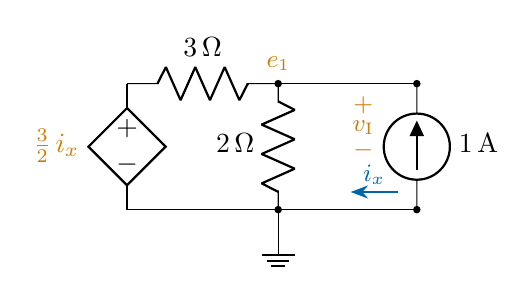
\begin{tikzpicture}[scale=0.8]
        \exR{1}
      \end{tikzpicture}
    \end{column}
    \begin{column}{0.48\textwidth}
      \small
      \textbf{Node 1:}\\[2pt]
      $\displaystyle \frac{\e{1} - \frac32\,\Icol{i_x}}{3} + \frac{\e{1}}{2} - 1 = 0$\\[10pt]
      \onslide<2->{%
      $\Icol{i_x} = \ ?$\\[4pt]}
      \onslide<3->{%
      $\Icol{i_x} = -1\A$\\[10pt]}
      \onslide<4->{%
      $\displaystyle \frac{\e{1} + \frac32}{3} + \frac{\e{1}}{2} - 1 = 0
      \ \Rightarrow\ \e{1} = \tfrac35\V$\\[12pt]}
      \onslide<5->{%
      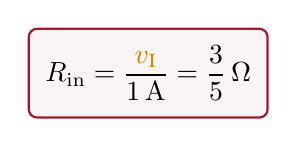
\begin{tikzpicture}
        \node[draw=metured, thick, fill=metured!5, rounded corners=3pt, inner sep=6pt]
          {$\displaystyle \Rin = \frac{\Vcol{v_{\mathrm{I}}}}{1\A} = \frac35\ohm$};
      \end{tikzpicture}}
    \end{column}
  \end{columns}
\end{frame}

%==============================================================
\roadmapframe{2}

%--------------------------------------------------------------
\begin{frame}{Three-terminal circuits: $\Delta$ and Y}
  \vfill
  \begin{center}
    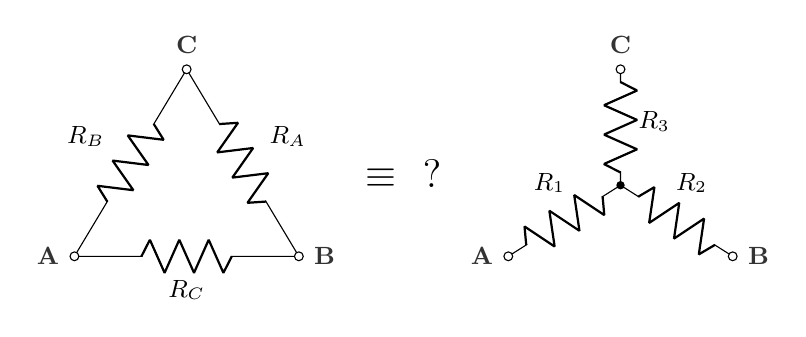
\begin{tikzpicture}[scale=0.95]
      \Dlt{0}
      \node[font=\Large] at (4.4,1.1) {$\equiv$ \ ?};
      \begin{scope}[shift={(5.8,0)}]
        \Wye{0}
      \end{scope}
    \end{tikzpicture}
  \end{center}
  \vfill
  \onslide<2->{%
  \begin{center}
    Given $R_A$, $R_B$, $R_C$: \ find $R_1$, $R_2$, $R_3$\\[6pt]
    \onslide<3->{The \alert{same resistance} between every two terminals}
  \end{center}}
  \vfill
\end{frame}

%--------------------------------------------------------------
\begin{frame}{$\Delta$ to Y: the resistance between two terminals}
  \begin{center}
    \begin{tikzpicture}[scale=0.62]
      \only<1>{\Dlt{1}}\only<2>{\Dlt{2}}\only<3->{\Dlt{3}}
      \begin{scope}[shift={(5.6,0)}]
        \only<1>{\Wye{1}}\only<2>{\Wye{2}}\only<3->{\Wye{3}}
      \end{scope}
    \end{tikzpicture}
  \end{center}
  \vspace{-4pt}
  \[
    \begin{array}{r@{\quad}c@{\quad}c@{\quad}l}
      & \Delta & & \mathrm{Y}\\[3pt]
      \text{A--B:} & \dfrac{R_C(R_A + R_B)}{\SD} & = & R_1 + R_2 \quad (1)\\[12pt]
      \onslide<2->{\text{B--C:}} & \onslide<2->{\dfrac{R_A(R_B + R_C)}{\SD}} & \onslide<2->{=} & \onslide<2->{R_2 + R_3 \quad (2)}\\[12pt]
      \onslide<3->{\text{C--A:}} & \onslide<3->{\dfrac{R_B(R_C + R_A)}{\SD}} & \onslide<3->{=} & \onslide<3->{R_3 + R_1 \quad (3)}
    \end{array}
  \]
\end{frame}

%--------------------------------------------------------------
\begin{frame}{$\Delta$ to Y: the result}
  \vfill
  \[
    \tfrac12\big[(1) + (2) + (3)\big]: \quad
    R_1 + R_2 + R_3 = \frac{R_A R_B + R_B R_C + R_C R_A}{\SD} \quad (4)
  \]
  \vfill
  \onslide<2->{%
  \[
    \Icol{R_1} = \frac{R_B R_C}{\SD} \ \ \text{\small (4)$-$(2)} \qquad
    \onslide<3->{\Icol{R_2} = \frac{R_C R_A}{\SD} \qquad
    \Icol{R_3} = \frac{R_A R_B}{\SD}}
  \]}
  \vfill
  \onslide<4->{%
  \begin{columns}[c,onlytextwidth]
    \begin{column}{0.42\textwidth}
      \centering
      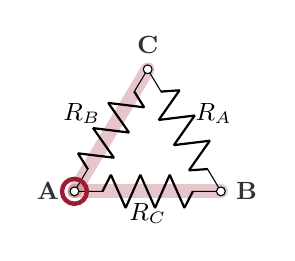
\begin{tikzpicture}[scale=0.62]
        \draw[sdel] (0,0) -- (1.5,2.5); \draw[sdel] (0,0) -- (3,0);
        \Dlt{0}
        \node[hterm] at (0,0) {};
      \end{tikzpicture}
    \end{column}
    \begin{column}{0.56\textwidth}
      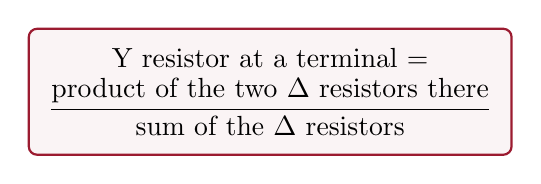
\begin{tikzpicture}
        \node[draw=metured, thick, fill=metured!5, rounded corners=3pt, inner sep=7pt, align=center]
          {Y resistor at a terminal $=$\\[3pt]
           $\dfrac{\text{product of the two $\Delta$ resistors there}}{\text{sum of the $\Delta$ resistors}}$};
      \end{tikzpicture}
    \end{column}
  \end{columns}}
  \vfill
\end{frame}

%--------------------------------------------------------------
\begin{frame}{Y to $\Delta$}
  \vfill
  Given $R_1$, $R_2$, $R_3$: \ find $R_A$, $R_B$, $R_C$
  \vfill
  \onslide<2->{%
  \[
    R_1 R_2 + R_2 R_3 + R_3 R_1 = \frac{R_A R_B R_C\,(\SD)}{(\SD)^2} = \frac{R_A R_B R_C}{\SD}
  \]}
  \vfill
  \onslide<3->{%
  \[
    R_A R_1 = R_B R_2 = R_C R_3 = \frac{R_A R_B R_C}{\SD}
  \]}
  \vfill
  \onslide<4->{%
  \[
    \textcolor{metured}{R_A} = \frac{R_1R_2 + R_2R_3 + R_3R_1}{R_1}, \qquad
    \textcolor{metured}{R_B} = \frac{\cdots}{R_2}, \qquad
    \textcolor{metured}{R_C} = \frac{\cdots}{R_3}
  \]}
  \vfill
  \onslide<5->{%
  \begin{center}
    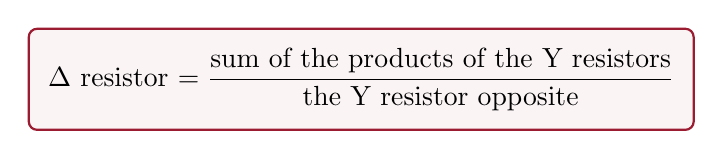
\begin{tikzpicture}
      \node[draw=metured, thick, fill=metured!5, rounded corners=3pt, inner sep=7pt]
        {$\Delta$ resistor $= \dfrac{\text{sum of the products of the Y resistors}}{\text{the Y resistor opposite}}$};
    \end{tikzpicture}
  \end{center}}
  \vfill
\end{frame}

%--------------------------------------------------------------
\begin{frame}{Equal resistors}
  \vfill
  \begin{center}
    \begin{tikzpicture}[scale=0.95]
      \Dltq
      \node[font=\Large] at (4.4,1.1) {$\equiv$};
      \begin{scope}[shift={(5.8,0)}]
        \only<1>{\Wyeq{\,?\,}}\only<2->{\Wyeq{R/3}}
      \end{scope}
    \end{tikzpicture}
  \end{center}
  \vfill
  \onslide<2->{%
  \begin{center}
    $\dfrac{R \cdot R}{3R} = \dfrac{R}{3}$ \qquad\qquad
    \onslide<3->{Y with $R$ \ $\equiv$ \ $\Delta$ with $3R$}
  \end{center}}
  \vfill
\end{frame}

%==============================================================
\roadmapframe{4}

%--------------------------------------------------------------
\begin{frame}{Example 13.2: a bridge}
  \vfill
  \begin{center}
    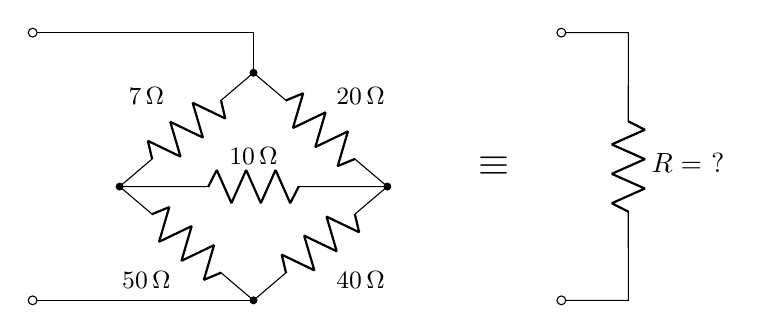
\begin{tikzpicture}[scale=0.85]
      \exBr{0}
      \node[font=\Large] at (5.6,2.0) {$\equiv$};
      \draw (6.6,4.0) node[ocirc] {} -- (7.6,4.0) to[R, l={$R = \ ?$}] (7.6,0) -- (6.6,0) node[ocirc] {};
    \end{tikzpicture}
  \end{center}
  \vfill
  \onslide<2->{\begin{center}No two resistors in series or in parallel\end{center}}
  \vfill
\end{frame}

%--------------------------------------------------------------
\begin{frame}{Example 13.2: $\Delta$ to Y}
  \begin{columns}[c,onlytextwidth]
    \begin{column}{0.5\textwidth}
      \centering
      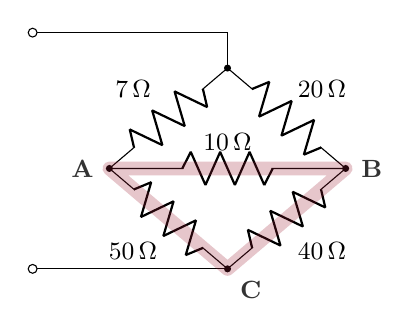
\begin{tikzpicture}[scale=0.75]
        \exBr{1}
      \end{tikzpicture}
    \end{column}
    \begin{column}{0.48\textwidth}
      $\Delta$ \ A--B--C:\\[4pt]
      $R_C = 10\ohm$, \ $R_B = 50\ohm$, \ $R_A = 40\ohm$\\[10pt]
      \onslide<2->{%
      $\SD = 100\ohm$\\[10pt]}
      \onslide<3->{%
      $\Icol{R_1} = \dfrac{50 \cdot 10}{100} = \Icol{5\ohm}$\\[6pt]
      $\Icol{R_2} = \dfrac{10 \cdot 40}{100} = \Icol{4\ohm}$\\[6pt]
      $\Icol{R_3} = \dfrac{40 \cdot 50}{100} = \Icol{20\ohm}$}
    \end{column}
  \end{columns}
\end{frame}

%--------------------------------------------------------------
\begin{frame}{Example 13.2: the new circuit}
  \begin{columns}[c,onlytextwidth]
    \begin{column}{0.5\textwidth}
      \centering
      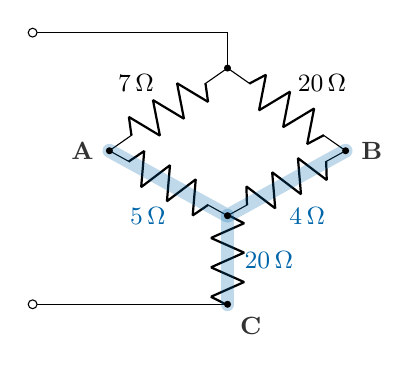
\begin{tikzpicture}[scale=0.75]
        \exBr{2}
      \end{tikzpicture}
    \end{column}
    \begin{column}{0.48\textwidth}
      Series: \ $7 + 5 = 12\ohm$, \quad $20 + 4 = 24\ohm$\\[10pt]
      \onslide<2->{%
      Parallel: \ $12 \parallel 24 = 8\ohm$\\[10pt]}
      \onslide<3->{%
      Series: \ $8 + 20$\\[12pt]
      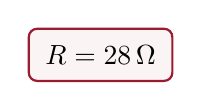
\begin{tikzpicture}
        \node[draw=metured, thick, fill=metured!5, rounded corners=3pt, inner sep=6pt]
          {$R = 28\ohm$};
      \end{tikzpicture}}
    \end{column}
  \end{columns}
\end{frame}

%--------------------------------------------------------------
\begin{frame}{Motivation: many sources}
  \vfill
  \begin{center}
    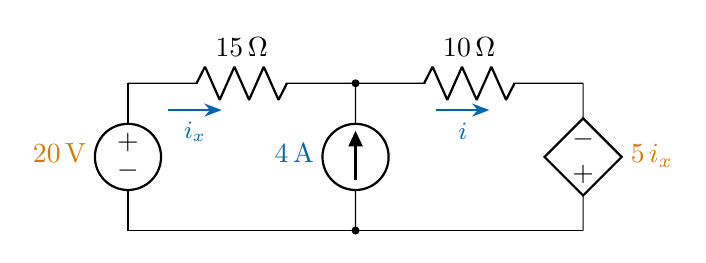
\begin{tikzpicture}[scale=0.85]
      \exS{0}
    \end{tikzpicture}
  \end{center}
  \vfill
  \begin{itemize}\itemsep8pt
    \item Two independent sources: the \alert{inputs}
    \item<2-> One source at a time: two simpler circuits?
    \item<3-> Yes: the circuit is \alert{linear}
  \end{itemize}
  \vfill
\end{frame}

%==============================================================
\roadmapframe{5}

%--------------------------------------------------------------
\begin{frame}{Linearity: inputs and outputs}
  \begin{columns}[c,onlytextwidth]
    \begin{column}{0.5\textwidth}
      \centering
      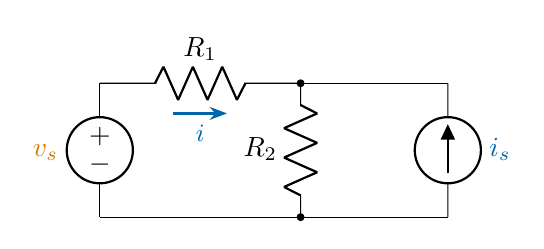
\begin{tikzpicture}[scale=0.85]
        \exL
      \end{tikzpicture}
    \end{column}
    \begin{column}{0.48\textwidth}
      \textbf{Input} vector: the independent sources\\[4pt]
      $\mathbf{u} = \begin{bmatrix} \Vcol{v_s}\\ \Icol{i_s} \end{bmatrix}$\\[14pt]
      \onslide<2->{%
      \textbf{Output} $y$: any branch voltage or current\\[4pt]
      e.g. $y = \Icol{i}$}
    \end{column}
  \end{columns}
\end{frame}

%--------------------------------------------------------------
\begin{frame}{Linearity}
  \vfill
  \begin{center}
    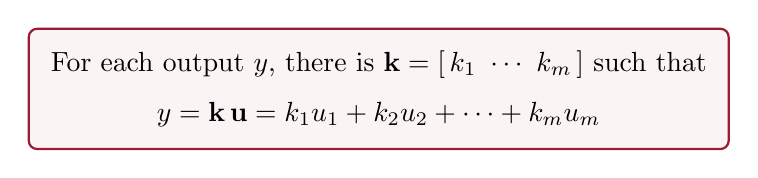
\begin{tikzpicture}
      \node[draw=metured, thick, fill=metured!5, rounded corners=3pt, inner sep=8pt, align=center]
        {For each output $y$, there is $\mathbf{k} = [\,k_1 \ \cdots \ k_m\,]$ such that\\[6pt]
         $y = \mathbf{k}\,\mathbf{u} = k_1u_1 + k_2u_2 + \cdots + k_mu_m$};
    \end{tikzpicture}
  \end{center}
  \vfill
  \onslide<2->{%
  \begin{center}
    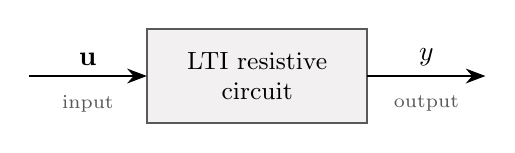
\begin{tikzpicture}
      \blockdiag
    \end{tikzpicture}\\[6pt]
    $y = y(\mathbf{u})$
  \end{center}}
  \vfill
\end{frame}

%--------------------------------------------------------------
\begin{frame}{Example 13.3: $\mathbf{k}$ for $y = \Icol{i}$}
  \begin{columns}[c,onlytextwidth]
    \begin{column}{0.5\textwidth}
      \centering
      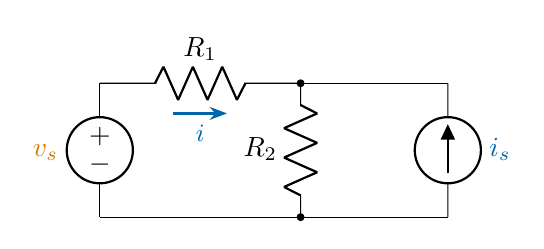
\begin{tikzpicture}[scale=0.85]
        \exL
      \end{tikzpicture}
    \end{column}
    \begin{column}{0.48\textwidth}
      $\Icol{i} = k_1\Vcol{v_s} + k_2\Icol{i_s}$: \ $k_1, k_2 = \ ?$\\[12pt]
      \onslide<2->{%
      \textbf{KVL:} \ $-\Vcol{v_s} + R_1\Icol{i} + R_2(\Icol{i} + \Icol{i_s}) = 0$\\[10pt]}
      \onslide<3->{%
      $\displaystyle \Icol{i} = \frac{1}{R_1 + R_2}\,\Vcol{v_s} - \frac{R_2}{R_1 + R_2}\,\Icol{i_s}$\\[12pt]}
      \onslide<4->{%
      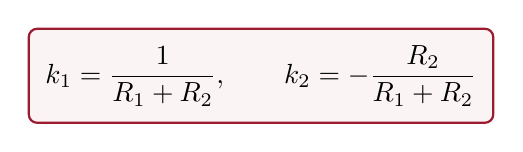
\begin{tikzpicture}
        \node[draw=metured, thick, fill=metured!5, rounded corners=3pt, inner sep=6pt]
          {$\displaystyle k_1 = \frac{1}{R_1 + R_2}, \qquad k_2 = -\frac{R_2}{R_1 + R_2}$};
      \end{tikzpicture}}
    \end{column}
  \end{columns}
\end{frame}

%--------------------------------------------------------------
\begin{frame}{Linearity: the implication}
  \vfill
  \begin{center}
    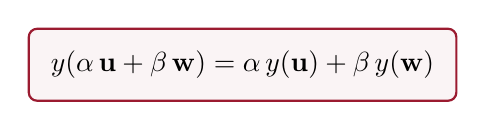
\begin{tikzpicture}
      \node[draw=metured, thick, fill=metured!5, rounded corners=3pt, inner sep=8pt]
        {$y(\alpha\,\mathbf{u} + \beta\,\mathbf{w}) = \alpha\,y(\mathbf{u}) + \beta\,y(\mathbf{w})$};
    \end{tikzpicture}\\[6pt]
    {\small $\mathbf{u}$, $\mathbf{w}$: input vectors; \ $\alpha$, $\beta$: numbers}
  \end{center}
  \vfill
  \onslide<2->{%
  \[
    y\!\left(\begin{bmatrix} \Vcol{v_s}\\ \Icol{i_s} \end{bmatrix}\right)
    = y\!\left(\begin{bmatrix} \Vcol{v_s}\\ 0 \end{bmatrix}\right)
    + y\!\left(\begin{bmatrix} 0\\ \Icol{i_s} \end{bmatrix}\right)
  \]}
  \vfill
  \onslide<3->{%
  \begin{center}
    \textbf{Superposition:} one independent source at a time
  \end{center}}
  \vfill
\end{frame}

%==============================================================
\roadmapframe{6}

%--------------------------------------------------------------
\begin{frame}{Killing a source}
  \vfill
  \begin{columns}[t,onlytextwidth]
    \begin{column}{0.47\textwidth}
      \begin{block}{Voltage source}
        \centering
        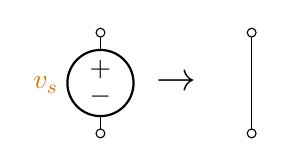
\begin{tikzpicture}[scale=0.8]
          \draw (0,1.6) node[ocirc] {} to[american voltage source, l_=$\Vcol{v_s}$] (0,0) node[ocirc] {};
          \node[font=\Large] at (1.2,0.8) {$\to$};
          \draw (2.4,1.6) node[ocirc] {} -- (2.4,0) node[ocirc] {};
        \end{tikzpicture}\\[4pt]
        $\Vcol{v_s} = 0$: \ a \alert{short circuit}
      \end{block}
    \end{column}
    \begin{column}{0.47\textwidth}
      \onslide<2->{%
      \begin{block}{Current source}
        \centering
        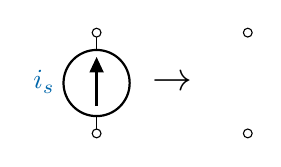
\begin{tikzpicture}[scale=0.8]
          \draw (0,0) node[ocirc] {} to[american current source, l=$\Icol{i_s}$] (0,1.6) node[ocirc] {};
          \node[font=\Large] at (1.2,0.8) {$\to$};
          \draw (2.4,1.6) node[ocirc] {}; \draw (2.4,0) node[ocirc] {};
        \end{tikzpicture}\\[4pt]
        $\Icol{i_s} = 0$: \ an \alert{open circuit}
      \end{block}}
    \end{column}
  \end{columns}
  \vfill
  \onslide<3->{%
  \begin{center}
    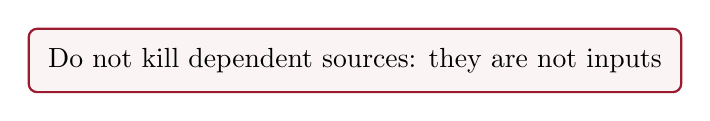
\begin{tikzpicture}
      \node[draw=metured, thick, fill=metured!5, rounded corners=3pt, inner sep=7pt]
        {Do \alert{not} kill dependent sources: they are not inputs};
    \end{tikzpicture}
  \end{center}}
  \vfill
\end{frame}

%--------------------------------------------------------------
\begin{frame}{Example 13.4: superposition}
  \vfill
  \begin{center}
    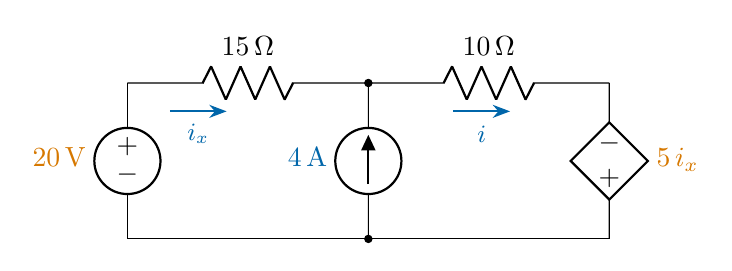
\begin{tikzpicture}[scale=0.9]
      \exS{0}
    \end{tikzpicture}
  \end{center}
  \vfill
  \begin{center}
    Find $\Icol{i}$, one source at a time\\[10pt]
    \onslide<2->{$\Icol{i} = \Icol{i_1} + \Icol{i_2}$: \quad
    $\Icol{i_1}$: only $20\V$, \quad $\Icol{i_2}$: only $4\A$}
  \end{center}
  \vfill
\end{frame}

%--------------------------------------------------------------
\begin{frame}{Example 13.4: kill the current source}
  \begin{columns}[c,onlytextwidth]
    \begin{column}{0.52\textwidth}
      \centering
      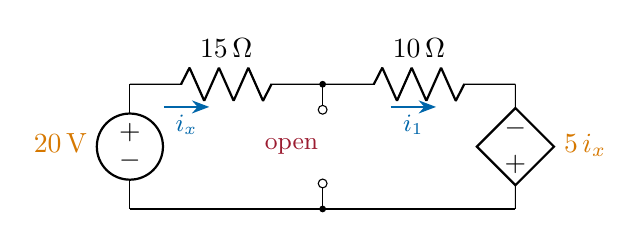
\begin{tikzpicture}[scale=0.72]
        \exS{1}
      \end{tikzpicture}
    \end{column}
    \begin{column}{0.46\textwidth}
      \textbf{KVL:}\\[2pt]
      $-20 + 15\,\Icol{i_x} + 10\,\Icol{i_1} - 5\,\Icol{i_x} = 0$\\[10pt]
      \onslide<2->{%
      $\Icol{i_x} = \ ?$\\[4pt]}
      \onslide<3->{%
      $\Icol{i_x} = \Icol{i_1}$ \ $\Rightarrow$ \ $20\,\Icol{i_1} = 20$\\[10pt]
      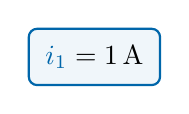
\begin{tikzpicture}
        \node[draw=ccur, thick, fill=ccur!6, rounded corners=3pt, inner sep=6pt]
          {$\Icol{i_1} = 1\A$};
      \end{tikzpicture}}
    \end{column}
  \end{columns}
\end{frame}

%--------------------------------------------------------------
\begin{frame}{Example 13.4: kill the voltage source}
  \begin{columns}[c,onlytextwidth]
    \begin{column}{0.52\textwidth}
      \centering
      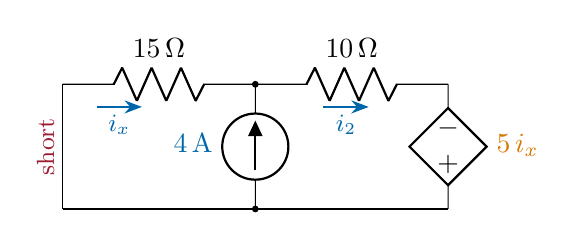
\begin{tikzpicture}[scale=0.72]
        \exS{2}
      \end{tikzpicture}
    \end{column}
    \begin{column}{0.46\textwidth}
      \textbf{KVL:}\\[2pt]
      $15\,\Icol{i_x} + 10\,\Icol{i_2} - 5\,\Icol{i_x} = 0$\\[10pt]
      \onslide<2->{%
      $\Icol{i_x} = \ ?$\\[4pt]}
      \onslide<3->{%
      $\Icol{i_x} = \Icol{i_2} - 4$ \ $\Rightarrow$ \ $20\,\Icol{i_2} = 40$\\[10pt]
      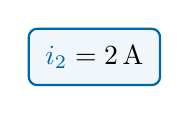
\begin{tikzpicture}
        \node[draw=ccur, thick, fill=ccur!6, rounded corners=3pt, inner sep=6pt]
          {$\Icol{i_2} = 2\A$};
      \end{tikzpicture}\\[12pt]}
      \onslide<4->{%
      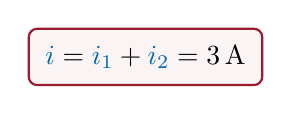
\begin{tikzpicture}
        \node[draw=metured, thick, fill=metured!5, rounded corners=3pt, inner sep=6pt]
          {$\Icol{i} = \Icol{i_1} + \Icol{i_2} = 3\A$};
      \end{tikzpicture}}
    \end{column}
  \end{columns}
\end{frame}

%==============================================================
\roadmapframe{7}

%--------------------------------------------------------------
\begin{frame}{Example 13.5: three experiments}
  \begin{center}
    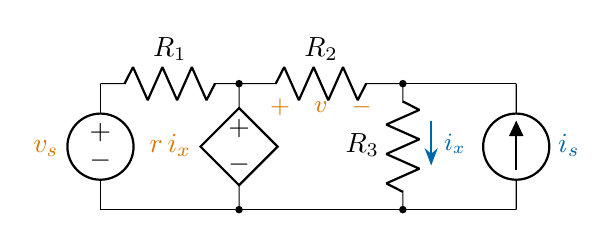
\begin{tikzpicture}[scale=0.8]
      \exT
    \end{tikzpicture}
  \end{center}
  \begin{columns}[c,onlytextwidth]
    \begin{column}{0.48\textwidth}
      \centering
      \renewcommand{\arraystretch}{1.2}
      \begin{tabular}{l|c|c|c}
        & $\Vcol{v_s}$ & $\Icol{i_s}$ & $\Vcol{v}$\\ \hline
        Exp.\ 1 & $12\V$ & $0$ & $\Vcol{v_1}$\\
        Exp.\ 2 & $-6\V$ & $6\A$ & $\Vcol{v_2}$\\
        Exp.\ 3 & $4\V$ & $4\A$ & $\Vcol{v_3}$
      \end{tabular}
    \end{column}
    \begin{column}{0.5\textwidth}
      $\Vcol{v_3}$ in terms of $\Vcol{v_1}$ and $\Vcol{v_2}$?\\[10pt]
      \onslide<2->{%
      Linearity: \ $\Vcol{v} = \mathbf{k}\begin{bmatrix} \Vcol{v_s}\\ \Icol{i_s} \end{bmatrix}$}
    \end{column}
  \end{columns}
\end{frame}

%--------------------------------------------------------------
\begin{frame}{Example 13.5: the solution}
  \vfill
  \[
    \begin{bmatrix} 4\\ 4 \end{bmatrix}
    = \alpha \begin{bmatrix} 12\\ 0 \end{bmatrix} + \beta \begin{bmatrix} -6\\ 6 \end{bmatrix}
    \onslide<2->{\qquad\Rightarrow\qquad \beta = \tfrac23, \quad \alpha = \tfrac23}
  \]
  \vfill
  \onslide<3->{%
  \[
    \Vcol{v_3} = \Vcol{v}\!\left(\alpha \begin{bmatrix} 12\\ 0 \end{bmatrix} + \beta \begin{bmatrix} -6\\ 6 \end{bmatrix}\right)
    = \alpha\,\Vcol{v_1} + \beta\,\Vcol{v_2}
  \]}
  \vfill
  \onslide<4->{%
  \begin{center}
    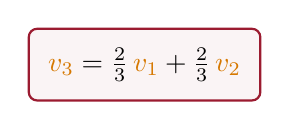
\begin{tikzpicture}
      \node[draw=metured, thick, fill=metured!5, rounded corners=3pt, inner sep=7pt]
        {$\Vcol{v_3} = \tfrac23\,\Vcol{v_1} + \tfrac23\,\Vcol{v_2}$};
    \end{tikzpicture}\\[8pt]
    No element values needed
  \end{center}}
  \vfill
\end{frame}

%--------------------------------------------------------------
\begin{frame}{Summary}
  \vfill
  \begin{center}
  \renewcommand{\arraystretch}{1.7}
  \begin{tabular}{@{}>{\raggedright}p{4.6cm} >{\raggedright\arraybackslash}p{7.6cm}@{}}
    \toprule
    \textbf{In the circuit} & \textbf{What to do}\\
    \midrule
    resistors, dependent sources & $\Rin = \Vcol{v}/1\A$ with a $1\A$ test source\\
    a $\Delta$ & Y: \ $R_1 = R_B R_C/(\SD)$, \dots\\
    a Y & $\Delta$: \ $R_A = (R_1R_2 + R_2R_3 + R_3R_1)/R_1$, \dots\\
    equal resistors & $\Delta$ with $R$ \ $\equiv$ \ Y with $R/3$\\
    linear circuit & $y = \mathbf{k}\,\mathbf{u}$: \ $y(\alpha\mathbf{u} + \beta\mathbf{w}) = \alpha y(\mathbf{u}) + \beta y(\mathbf{w})$\\
    several sources & superposition: \ killed $\Vcol{v_s}$ = short, \ killed $\Icol{i_s}$ = open\\
    \bottomrule
  \end{tabular}
  \end{center}
  \vfill
\end{frame}

\end{document}
